\documentclass{article}
\usepackage{amsfonts, amsmath, amssymb, amsthm} % Math notations imported
\usepackage{enumitem}
\usepackage{graphicx}
\usepackage[margin=1in]{geometry}
\usepackage{setspace}
\graphicspath{{./images/}} % Path to images

% \begin{figure}[htb!]
%      \centering
%      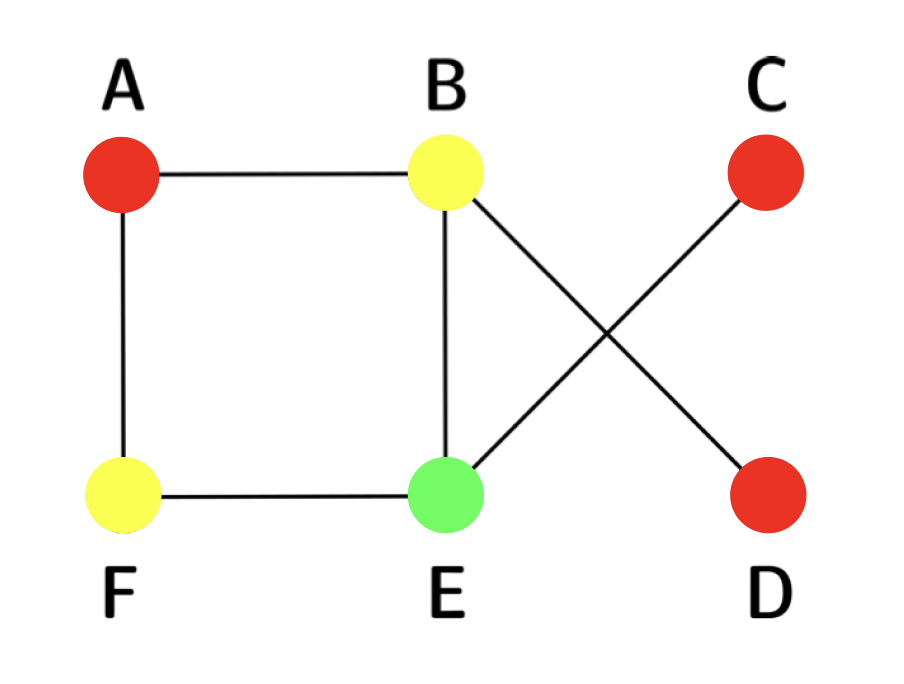
\includegraphics[scale=0.5]{coloring.png}
%      \caption{Coloring of the graph.}
% \end{figure}

\newtheorem{thm}{Theorem}
\newtheorem{proposition}[thm]{Proposition}
\newtheorem{cor}[thm]{Corollary}

% title information
\title{Math 128A HW1}
\author{Neo Lee}
\date{09/06/2023}

\setstretch{1.15}
% main content
\begin{document} 

% placing title information; comment out if using fancyhdr
\maketitle 

\section*{Section 1.1}
\subsection*{Problem 2c}
\begin{proposition}
    $f(x) = -3\cdot tan(2x) + x = 0$ has at least one solution for $x \in [0,1]$.
\end{proposition}
\begin{proof}
    Note that the interval is end point inclusive. 
    We have $f(0) = 0$, which is immediately one solution to the equation.
\end{proof}

\subsection*{Problem 2d}
\begin{proposition}
    $f(x) = ln(x)-x^2+\frac{5}{2}x - 1 = 0$ has at least one solution for $x \in [\frac{1}{2},1]$.
\end{proposition}
\begin{proof}
    $f(\frac{1}{2}) \approx -0.693, f(1) = 0.5$. Hence, by the intermediate value theorem, there 
    exists a solution in the interval.
\end{proof}

\subsection*{Problem 4d}
Find interval containing solutions to $x^3 + 4.001x^2 + 4.002x + 1.101 = 0$.

\subsection*{Problem 6a}
Find $max_{a\le x\le b}|f(x)|$ for $f(x) = \frac{2x}{x^2+1}$ on $[0,2]$.
\begin{proof}[Solution]
    We proceed by finding the critical points of $f(x)$ on $[0,2]$.

    \begin{align*}
        f'(x) & = \frac{2(x^2+1) - 2x(2x)}{(x^2+1)^2} \\
              & = \frac{2 - 2x^2}{(x^2+1)^2} \\
              & = 0 \text{ when } x = \pm 1.
    \end{align*}

    Then, we have $f(0) = 0, f(1) = 1, f(2) = \frac{4}{5}$. Hence, the maximum value of $f(x)$ on 
    $[0,2]$ is $1$ when $x=1$.
\end{proof}

\subsection*{Problem 14}
Let $f(x) = 2x\cdot cos(2x) - (x-2)^2$ and $x_0 = 0$.
\begin{enumerate}[label=(\alph*)]
    \item Find the third Taylor polynomial $P_3(x)$ and use it to approximate $f(0.4)$.
    \begin{proof}[Solution]
        \begin{align*}
            f'(x) & = 2cos(2x) - 4xsin(2x) - 2(x-2), \\
            f''(x) & = -8sin(2x) - 8xcos(2x) - 2 \\
            f'''(x) & = 16xsin(2x) - 24cos(2x).
        \end{align*}

        Now, we have $f(0) = -4, f'(0) = 6, f''(0) = -2, f'''(0) = -24$. Hence, the third Taylor 
        polynomial $P_3(x) = -4 + 6x -x^2 -4x^3$, and $f(0.4) \approx -2.016$.
    \end{proof}

    \item Use the error formula in Taylor's Theorem to find an upper bound for the error 
    $|f(0.4) - P_3(0.4)|$

    \begin{proof}[Solution]
        \begin{align*}
            f^4(x) & = 64sin(2x) + 32xcos(2x) \\
            R_3(x) & = \frac{f^4(\xi(x))}{4!}(0.4)^4 \qquad \emph{for } 0 \le \xi(x) \le 0.4.
        \end{align*}

        Hence, \begin{align*}
            |f(0.4) - P_3(0.4)| = |R_3(0.4)| & = \frac{f^4(\xi(x))}{4!}(0.4)^4 \\
            & = \frac{64sin(2\xi(x))-32\cdot \xi(x)cos(2\xi(x))}{24}\times 0.0256 \\
            & \le \frac{64-32\cdot \xi(x)}{24}\times 0.0256 \qquad (\emph{notice } 0 \le sin(2\xi(x)),
            cos(2\xi(x))\le 1)\\
            & \le \frac{64}{24}\times 0.0256 \\
            & \le 0.06827.
        \end{align*}
    \end{proof}
\end{enumerate}

\subsection*{Problem 26} 
Note that the variable $n-1$ needs to be replace by $n$.

\section*{Section 1.2}
\subsection*{Problem 2c}
\subsection*{Problem 4b}
\subsection*{Problem 12}
\subsection*{Problem 22}

\section*{Section 1.3}
\subsection*{Problem 8}
\subsection*{Problem 15}
\subsection*{Discussion Question 2 (p. 38)}

\section*{Section 2.1}
\subsection{Problem 6d}
\subsection{Problem 8}
\subsection{Problem 20}

\end{document}
